\noindent
\begin{tabular}{cc}
\begin{minipage}{0.60\textwidth}
\begin{exerciseS}[Gomito]
Un condotto di sezione circolare avente diametro $D = 5\ cm$ 
forma un gomito con angolo di $90^\circ$. Nel condotto scorre acqua ($\rho = 
999\ kg/m^3$) in regime stazionario con velocità $V = 
0.5\ rm m/s$. All'esterno del condotto vi è atmosfera con 
pressione uniforme $P_{atm}=101325\ Pa$; inoltre le pressioni 
all'ingresso e all'uscita del gomito sono uniformi sulla sezione ed 
entrambe pari a $P=10^6\ Pa$. Calcolare la forza $\bm{F}$ agente 
sul gomito.\\
($\bm{F} = -1765.03\hat{\bm{x}} + 1765.03\hat{\bm{y}}\  N$)
\end{exerciseS}
\end{minipage}
&
\begin{minipage}{0.35\textwidth}
   \begin{center}
   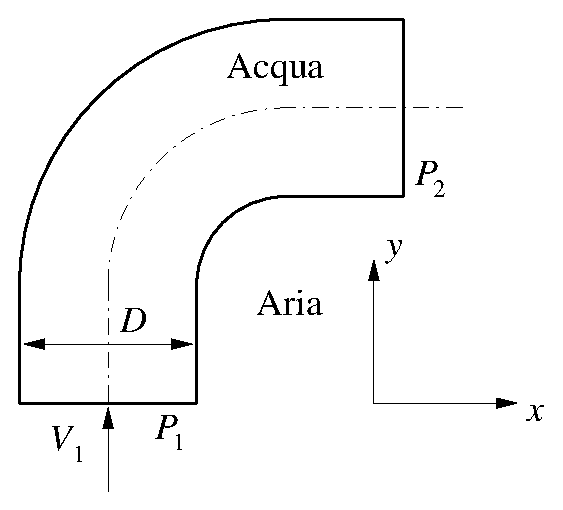
\includegraphics[width=0.70\textwidth]{./fig/gomito_01.eps}
   \end{center}
\end{minipage}
\end{tabular}


\sol

\partone
 Bilanci integrali di massa e quantità di moto. ...
\begin{equation}
\begin{cases}
  \frac{d}{dt} \int_V \rho = -\oint_{\partial V} \rho \bm{u} \cdot \hat{\bm{n}}  & \text{(massa)} \\
  \frac{d}{dt} \int_V \rho \bm{u} = -\oint_{\partial V} \rho \bm{u} \bm{u} \cdot \hat{\bm{n}}
  +\int_V \bm{F} - \oint_{\partial V} p \hat{\bm{n}} + \oint_{\partial V} {\bm{s_n}} & \text{(quantità di moto)}
\end{cases}
\end{equation}

\parttwo
Vengono fatte alcune ipotesi: regime stazionario, fluido incomprimibile, fluido non viscoso, profili costanti di velocità, no gravità.
Si scrivono i bilanci integrali semplificati, si riconoscono in essi e si calcolano le azioni scambiate con il corpo.

\begin{itemize}
  \item Scrittura dei bilanci integrali opportunamente semplificati (ipotesi).
    \begin{equation}
     \begin{cases}
      \oint_{\partial V} \rho \bm{u} \cdot \hat{\bm{n}} = 0  & \text{(massa)} \\
      \oint_{\partial V} \rho \bm{u} \bm{u} \cdot \hat{\bm{n}} = \oint_{\partial V} \bm{t_n} & \text{(quantità di moto)}
     \end{cases}
    \end{equation}
  \item Ulteriore semplificazione usando l'ipotesi di densità costante e profili di velocità uniformi
    \begin{equation}
     \begin{cases}
      -V_1 A_1 + V_2 A_2 = 0 \qquad \qquad \qquad \Rightarrow  V_1 = V_2 = V \\
      - \rho \vec{V_1} V_1 A_1 + \rho \vec{V_2} V_2 A_2 = \oint_{\partial V} \bm{t_n}
     \end{cases}
    \end{equation}
  \item Relazione tra l'integrale degli sforzi sulla superficie e la risultante delle forze agenti sul gomito, sfruttando il fatto che l'integrale della normale su tutta la superficie è identicamente nullo. Si identificano con $S_1$ la superficie di ingresso, $S_2$ la superficie di uscita, $S_3$ la superficie laterale.
    \begin{equation}
     \begin{aligned}
       \displaystyle\oint_{S_1\cup S_2\cup S_3} \bm{t_n} & =  \displaystyle\oint_{S_1\cup S_2\cup S_3} \bm{t_n} + \underbrace{\displaystyle\oint_{S_1\cup S_2\cup S_3} p_a \hat{n}}_{=0} = \\
      & = -\oint_{S_1} (p-p_a) \hat{n} - \oint_{S_2} (p-p_a) \hat{n} + \underbrace{\oint_{S_3} (\bm{t_n}+p_a \hat{n})}_{=-\bm{F}} =  \\
      & = -\oint_{S_1} (p-p_a) \hat{n} - \oint_{S_2} (p-p_a) \hat{n} - \bm{F} 
     \end{aligned}
    \end{equation}
  \item Proiezione lungo i due assi del sistema di riferimento della risultante delle forze agenti sul gomito (dopo averla inserita nell'equazione di bilancio della quantità di moto)
\begin{equation}
  \begin{cases}
    F_x = - \rho V^2 A - (p_2 - p_a)A   \\
    F_y =  \rho V^2 A + (p_1 - p_a)A  
  \end{cases}
  \end{equation}
%  \begin{equation}
%  \begin{cases}
%    F_x = - \rho V^2 A - (p_2 - p_a)A & \quad \Rightarrow \quad   F_x = -1765.03 N  \\
%    F_y =  \rho V^2 A + (p_1 - p_a)A  & \quad \Rightarrow \quad   F_y =  1765.03 N
%  \end{cases}
%  \end{equation}
\end{itemize}
